\section{Příklad 2}
\druhyZadani{H}

\begin{enumerate}
    \item \textbf{Seriové zapojení rezistorů $R_4$, $R_5$:} \newline
    $R_{45} = R_4 + R_5 = 205\Omega + 560\Omega = 765\Omega$
    
    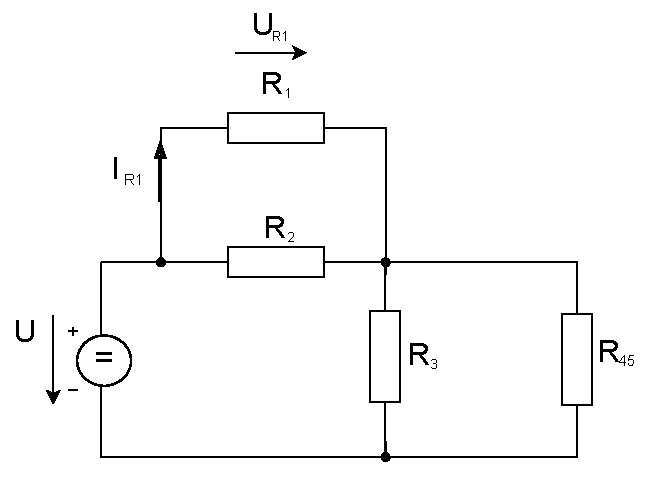
\includegraphics[scale=0.7]{pr2/pr2.1.pdf}
    
    \item \textbf{Paralelní zapojení rezistorů $R_3$, $R_{45}$:} \newline
    $R_{345} = \frac{R_3 * R_{45}}{R_3 + R_{45}} = \frac{580\Omega * 765\Omega}{580\Omega + 765\Omega} = \frac{443700\Omega}{1345\Omega} = 329,8885\Omega$
    
    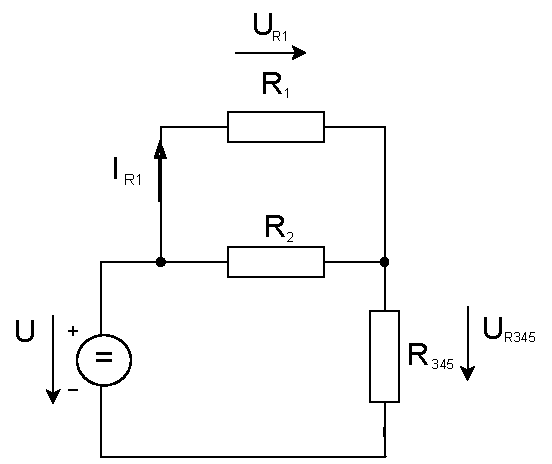
\includegraphics[scale=0.7]{pr2/pr2.2.pdf}
    
    \item \textbf{Použijeme Théveninůvu větu na $R_1$:} \newline
    $I_0 = \frac{U}{R_2 + R_{345}} = \frac{220V}{360\Omega + 329,8885\Omega} = \frac{220V}{689,8885\Omega} = 0,3189A$
    
    \item \textbf{Zjistíme odpor $R_i$ bez $R_1$:} \newline
    $R_i = \frac{R_2 * R_{345}}{R_2 + R_{345}} = \frac{360\Omega * 329,8885\Omega}{360\Omega + 329,8885\Omega} = \frac{118759,86\Omega}{689,8885\Omega} = 172,1436\Omega$
    
    \item \textbf{Zjistíme napětí $U_{345}$:} \newline
    $U_{345} = I_0 * R_{345} = 0,3189A * 329,8885\Omega = 105,2014V$
    
    \item \textbf{Zjistíme napětí zdroje bez $R_1$:} \newline
    $U_{AB} = U - U_{345} = 220V - 105,2014V = 114,7986V$
    
    \item \textbf{Zjistíme $I_{R1}$:} \newline
    $I_{R1} = \frac{U_{AB}}{R_i + R_1} = \frac{114,7986V}{172,1436\Omega + 190\Omega} = \frac{114,7986V}{362,7436\Omega} = 0,3165A$
    
    \item \textbf{Zjistíme napětí $U_{R1}$:} \newline
    $U_{R1} = I_{R1} * R_1 = 0,3165A * 190\Omega = 60,135V$
\end{enumerate}